\documentclass[11pt,oneside,a4paper]{article}     % onecolumn (second format)
\usepackage[T1]{fontenc}
\usepackage[english]{babel}
\usepackage[utf8]{inputenc}
\usepackage{epstopdf}
% GRAPHICS AND IMAGES

\usepackage{mathtools}
\usepackage{acronym}
\usepackage{graphicx}
\usepackage{amsthm}
\usepackage{amsmath}
\usepackage{amssymb}
\usepackage{tabularx}
\usepackage[algoruled, vlined, linesnumbered]{algorithm2e}% http://ctan.org/pkg/algorithms
%\usepackage{algpseudocode}
% INCLUDE YOUR PACKAGES HERE
%\usepackage{amsfonts,amsmath,amsthm, amssymb}
\usepackage{subfig}
\usepackage[font=scriptsize]{caption}
\usepackage[dvipsnames]{xcolor}
\newcommand*{\dt}[1]{\accentset{\mbox{\large\bfseries .}}{#1}}

\newcommand{\ind}{1{\hskip -2.5 pt} \mathrm{I}}


\newtheorem{definition}{Definition}
\newtheorem{lemma}{Lemma}
\newtheorem{prop}{Proposition}
\newtheorem{assumption}{Assumption}
\newtheorem{theorem}{Theorem}
\newtheorem{remark}{Remark}
\newtheorem{corollary}{Corollary}

\newenvironment{sistema}%
{\left\lbrace\begin{array}{@{}l@{}}}%
{\end{array}\right.}

\DeclareMathOperator*{\argmax}{arg\,max}
\DeclareMathOperator*{\argmin}{arg\,min}

\title{Max-min fair tutor-student assignment\\under lexicographic preferences}

\date{\today}
\author{MegaMath4SmallBiz}


\begin{document}
\maketitle


\section{Scenario}

Let $S,T$ be the set of students and tutors, respectively. For each student/tutor pair $(s, t)$ there exists a score $r_{s,t}$ that measures the affinity between student $s$ and tutor $t$.

Each tutor $t$ can mentor at most $N_t$ students. On the contrary, there is no bound on the number of tutors that can mentor the same student. More formally, let $x_{s,t}=\{0,1\}$ be the binary variable that equals 1 if and only if tutor $t$ is assigned to student $s$. Then, 
\begin{equation} \label{eq:constr1}
\sum_{s\in S} x_{s,t} \le N_t, \qquad \forall\, t\in T.
\end{equation}



\subsection{Related works}

If each tutor can only mentor exactly one student ($N_t=1$ for all $t\in T$) then our problem is similar to the one studied in \cite{santaclaus06} and  \cite{chakrabarty2009allocating}. 



\section{Desiderata}

We wish to find a tutor-student assignment $x^*$ with the following desiderata:
\begin{enumerate}
\item $x^*$ must respect constraint (\ref{eq:constr1}), i.e., each tutor $t$ cannot supervise more than $N_t$ students;
\item $x^*$ must take into account that student preferences are not linear in the affinities $r$ with the assigned tutors. For instance, a student $s$ arguably prefers to be assigned to a single tutor $t$ with score $10$ ($r_{s,t}=10$) rather than to two tutors with score equal to 5 each;
\item $x^*$ must be somehow ``fair'', thus it should intuitively avoid stark disparity among students. For instance, attempting to maximize the sum of affinities over all students and tutors is in general a bad idea since it does not guarantee fairness.
\end{enumerate}



\section{Preliminaries: max-min fairness}

We first observe that attempting at maximizing the total reward over all students is in general not a good idea since it generates stark inequalities among students. In fact, the solution in this case is to let each tutor $t$ choose the $N_t$ students with the highest affinity. In other words, each tutor $t$ ranks the students according to decreasing score $r_{s_1,t}\ge r_{s_2,t} \ge \dots$ and selects the first $N_t$ of them. However, there may be students with very low reward; potentially, there may be students $s$ with no tutors is assigned to them.


For the reason outlined above, we aim at finding a ``fair'' assignment between students and tutors. To this aim, let us first define the crucial concept of max-min fairness.

\begin{definition}[Max-min fair allocation] \cite{nace2008max}
An allocation $a^*$ is max-min fair when the only way to increase the reward $a_s^*$ of a student $s$ is by decreasing the reward of a students $s'$ with lower reward, i.e., such that $x^*_{s'}< x^*_{s'}$.
\end{definition}

We remark that the max-min fair allocation can be equivalently defined as the one achieving the lexicographic sorted optimum\footnote{Let $\overline{R}$ be the vector $R$ sorted in increasing order. We say that $R$ is preferred to $R'$ if $\overline{R}$ is lexicographically greater than $\overline{R}'$, i.e., $\exists \, n$ such that $\overline{R}_i=\overline{R}'_i$ for $i=1,\dots,n$ and $\overline{R}_{n+1}>\overline{R}'_{n+1}$.}.

Max-min fairness always give priority to students with smaller affinity with tutors (that would end up with a poor reward if we simply maximized the sum of rewards), and try to maximize their reward in an iterative fashion.






\section{Proposed solution: Iterative Max-Min}

We now describe our solution to assign fairly tutors to students, by exploiting the concept of max-min fairness.

The first idea is to apply the concept of max-min fairness to the sum of affinities between each student and all the tutors assigned to her. On the other hand, this would lead to a solution that does not well adapt to desiderata 2.

Therefore, we propose an algorithm that iteratively assigns one tutor to each student in a max-min fashion, as long as the constraints on the maximum number of students supervised by the tutors is fulfilled. By assigning only one tutor at the time, we tend to ensure high individual affinity for all students for the very first few iterations, which is in line with desiderata 3.

The main procedure can be resumed as follows.


\begin{algorithm}[H]
 \KwData{Students $S$, tutors $T$, student-tutor score $r_{s,t}$}
 \KwResult{Max-min fair student-tutor assignment $\tau$. \\ $\tau(s)\subset T$ is the set of tutors assigned to student $s$, for all $s\in S$.}
\textbf{Initialization}: Set $\tau(s)=\emptyset$ for all $s\in S$ and $S''=\emptyset$, containing the set of unassigned students. \\
\While{$\exists \, t: \, N_t>0$}{
Set $S':=S\setminus S''$.\\
\While{$(S'\ne \emptyset) \land (\exists \, t: \, N_t>0)$}{
Use dichotomy search Algorithm \ref{alg:dichot} to solve the following Core Problem CP:
\begin{equation} \label{eq:maxmin1}
\begin{sistema}
\widetilde{x}\, = \argmax_{x} \, y \\
\mathrm{s.t.} \, \sum_{t\in T_s} x_{s,t} \, r_{s,t} \ge y \qquad \forall\, s\in S' \\
\hspace{.67cm} \sum_{t\in T_s} x_{s,t} \le 1 \qquad \forall\, s\in S' \\
\hspace{.67cm} \sum_{s} x_{s,t} \le N_t \qquad \forall\, t\in T \\
\hspace{.67cm} x_{s,t} \in \{0,1\}, \qquad \forall\, s\in S',t\in T.
\end{sistema} \tag{CP}
\end{equation}\\
\If{\textnormal{CP is unfeasible}}{
Let $S^u$ be the set of unassigned students. Set $S':=S'\setminus S^u$ and $S'':=S''\cup S^u$.
}
\Else{Let $A=\{(\underline{s},\underline{t})\}$ be the assignments produced by Algorithm \ref{alg:dichot}. Assign the tutors to the students accordingly: $\tau(\underline{s}):=\tau(\underline{s})\cup \underline{t}$, $\forall\, (\underline{s},\underline{t})\in A$. \\
Update the set of students yet to be assigned to a tutor: $S':=S'\setminus \{\underline{s}:(\underline{s},\underline{t})\in A\}$.\\
Update the number of available slots for each tutor $\underline{t}$: $N_t:=N_t-|\{\underline{s}:(\underline{s},\underline{t})\in A\}|$.\\
Update the set of available tutors for each student: $T_{\underline{s}}:=T_{\underline{s}}\setminus \underline{t}$, where $(\underline{s},\underline{t})\in A$}
}}
\caption{Iterative Max-Min fair tutor-student assignment}
\label{alg:maxmin}
\end{algorithm}



\subsection{Dichotomy search}

We now discuss how to solve \ref{eq:maxmin1}. Our idea is to perform a dichotomy search on the value $u$, hence pruning all student-tutor connections with reward $r$ inferior to the current value of $u$. Then, the problem boils down to a special set cover problem on the set of students.\\



\begin{algorithm}[H]
% \KwData{Students $S$, tutors $T$, student-tutor score $r_{s,t}$}
 \KwResult{Optimal value $\widetilde x$ of \ref{eq:maxmin1}}
\textbf{Initialization}: Rank the scores $\{r_{s,t}\}_{s\in S',t\in T_s}$ in increasing order and form the vector $\bar r_1,\bar r_2,\dots,\bar r_M$, where $M=\sum_{s\in S'}|T_s|$. Set $l=1$ and $u=M$. Define $\mathcal P(a)=\{(s,t), s\in S',t\in T_s: \, r_{s,t}\ge a\}$. Then, denote by FP($a$) the following Feasibility Problem:
\begin{equation} \label{eq:setcover2}
\begin{sistema}
\sum_{t:(s,t)\in \mathcal P(a)} x_{s,t}= 1, \qquad \forall \, s\in S' \\
\sum_{s:(s,t)\in \mathcal P(a)} x_{s,t} \le N_t, \qquad \forall\, t\in T \\
x_{s,t}\in \{0,1\}, \qquad \forall\, (s,t)\in \mathcal P(a).
\end{sistema} \tag{FP($a$)}
\end{equation}\\
Solve FP($r_l$) via max-flow Algorithm \ref{alg:maxflow}. Let $S^u$ be the set of unassigned students.\\
\If{\textnormal{FP($r_l$) is unfeasible}}{
\textbf{Return} \emph{unfeasible} and the set of unassigned students $S^u$.}
Solve FP($r_u$) via max-flow Algorithm \ref{alg:maxflow}.\\
\If{\textnormal{FP($r_u$) is feasible}}{
\textbf{Return} the student-tutor assignments with maximum score: $A=\{(\underline{s},\underline{t}): \, r_{\underline{s},\underline{t}}=r_h\}$}
\While{$|u-l|>1$}{
Set $h=\lceil \frac{l+u}{2}\rceil$.\\
Solve FP($r_h$) via max-flow Algorithm \ref{alg:maxflow}.
\\
\If{\textnormal{FP($r_h$) is feasible}}{
Set $l:=h$.
}
\Else{
Set $r:=h$.
}}
\textbf{Return} the student-tutor assignment with lowest score: $A=\{(\underline{s},\underline{t}): \, r_{\underline{s},\underline{t}}=r_l\}$.
\caption{Dichotomy search for \ref{eq:maxmin1}}
\label{alg:dichot}
\end{algorithm}


\subsection{Max-flow for determining feasibility of FP}


We are only left with solving the feasibility problem FP($a$), that ask whether it is possible to assign at least one tutor to all students only using the student-tutor pairs with affinity at least $a$.

We next show that the problem can be converted into a Max-Flow problem, that can be solved via classic max-flow algorithms (note: the output must be integer).

\begin{algorithm}[H]
\KwResult{Determines whether Feasibility Problem FP$(a)$ is feasible; if not, it returns the set of unassigned students.}
Define the following capacitated undirected graph. Let $i$ be the source node, connected to each tutor $t\in T$ through edge $(i,t)$ having capacity $N_t$. Each tutor $t$ is connected to student $s$ whenever $(s,t)\in \mathcal P(a)$, via edge $(t,s)$ with unitary capacity. Each student $s\in S'$ is connected to the destination node $j$ through edge $(s,j)$ with unitary capacity.\\
Find an integer solution to the \texttt{max-flow} problem from $i$ to $j$ via the Ford-Fulkerson algorithm. Let $f^*$ be the optimal flow allocation and $F^*$ the optimal value.\\
\If{$F^*==|S'|$}{\textbf{Return} \emph{feasible}, the optimal flow allocation $f^*$ and the set of unassigned students $S^u=\emptyset$.}
\Else{\textbf{Return} \emph{unfeasible}, the optimal flow allocation $f^*$ and the set of unassigned students $S^u=\{s:f^*_{s,j}=0\}$.}
\caption{Max-flow for FP($a$)}
\label{alg:maxflow}
\end{algorithm}


\begin{figure}
\centering
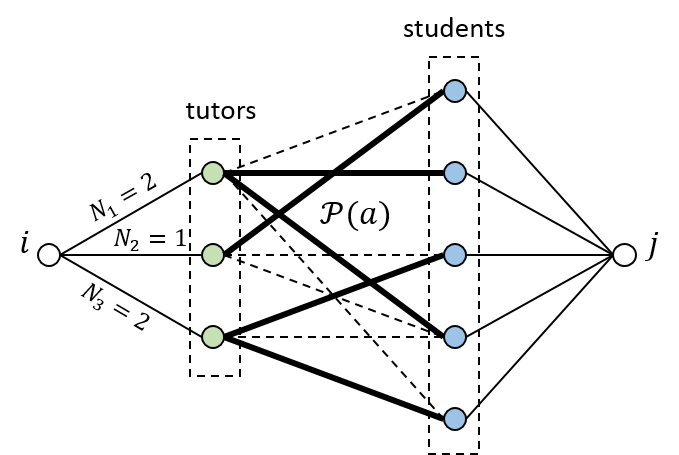
\includegraphics[scale=.75]{figs/maxflow.png}
\caption{Illustration of Algorithm \ref{alg:maxflow}, solving the \texttt{max-flow} problem from $i$ to $j$ associated to the graph induced by the tutor-student pairs $\mathcal P(a)$ with affinity not smaller than $a$. The edges from source $i$ to tutor $t$ has an annotated capacity $N_t$. All the other edges have unitary capacity. In this case, FP($a$) is feasible and the edges in bold constitute an optimal solution for FP($a$).}
\end{figure}



We now show that FP($a$) is a polynomial-time algorithm.

\begin{theorem}
Assume that $N_t$ is bounded for all possible instances. Then, max-flow Algorithm \ref{alg:maxflow} solves the Feasibility Problem \textnormal{FP($a$)} in polynomial time.
\end{theorem}

\begin{proof}
It is known that the max-flow problem can be solved by the Ford-Fulkerson algorithm in pseudo-polynomial time $\mathcal O (U(\mathrm{\#nodes+\#edges}))$, where $U$ upper bounds the network capacity \cite{ahuja2014network}. Then, if $N_t$ is bounded by $M>0$ then $U<M$ too, then the time is fully polynomial. Also, Ford-Fulkerson algorithm finds an integral flow whenever the capacities are integers. Then, we are left to prove that Algorithm \ref{alg:maxflow} solves FP($a$). In other words, we need to show that the solution of the max-flow problem in Algorithm \ref{alg:maxflow} outputs value $|S'|$ if and only if FP($a$) is feasible.

Assume first that FP($a$) is feasible and let us denote $\hat x$ a feasible solution. Then, assign a unitary flow $f_{t,s}$ on all edges $(t,s)$ such that $\hat x_{s,t}=1$. Assign flow $f_{i,t}=\sum_{s:(s,t)\in \mathcal P(a)} \hat x_{s,t}\le N_t$ to the edge $(i,t)$ (of capacity $N_t$), for each $t\in T$. 
Finally, assign flow $f_{s,j}=1$ to all edges of the form $(s,j)$, for all $s\in S'$. The flow $f$ is by construction a feasible flow from $i$ to $j$ in the graph defined in Algorithm \ref{alg:maxflow}. also, its value $F$ equals $S'$. We notice that its value equals the capacity of the cut between destination $j$ and the remaining nodes. Then, $F$ is maximum since the value of any feasible flow is never greater than the capacity of a graph cut.

Conversely, assume that $F^*=|S'|$ is the optimal value of the max-flow problem and let $f$ be the optimal integer flow allocation. Note first that $f_{s,j}=1$ for all $s\in S'$. By the integral flow theorem (see \cite{ahuja2014network}, Thm. 6.5), since all capacities are integer ($N_t$ or 1) then there exists an optimal integral flow allocation $f$. By flow conservation at node $s$, we have $\sum_{t:(s,t)\in \mathcal P(a)} f_{t,s}=f_{s,j}=1$. Also, the flow conservation at node $t$ and the capacity constraint on edge $(i,t)$ impose that $\sum_{s:(s,t)\in \mathcal P(a)} f_{t,s}=f_{i,t}\le N_t$. It is now easy to check that by setting $\hat x_{s,t}=f_{t,s}$, $\hat x$ is a feasible solution for FP($a$).
\end{proof}



\begin{corollary}
Iterative Max-min Algorithm \ref{alg:maxmin} has polynomial-time complexity.
\end{corollary}



\subsection{ToDOs}

The proposed algorithm provides the max-min allocation only if all affinities are different, i.e., $r_{s,t}\ne r_{s',t'}$ for all $s\ne s',t\ne t'$. The key is line 7 of Algorithm 2 that needs to be refined.

\section{Online assignment}

As time goes by, some students may depart and/or new students may subscribe to the platform, so the tutor-student assignment must be modified in a online fashion in order to deal with the new situation.

We have fundamentally two ways to deal with this online scenario.
The optimal way is to recompute from scratch the overall new tutor-student assignment, by taking into account the new situation. 

However, recomputing a new allocation from scratch may be too time costly, as we may need to provide a decent choice to a student that logs in for the first time. For this reason, we will devise a method to recompute the max-min allocation on a restricted subset of students, comprising the newly subscribed one.

We finally remark that, when a new allocation is computed, the only student-tutor pair assignments that need to be maintained are those who currently have an ongoing conversation.




\bibliographystyle{plain}
\bibliography{bib_frateli}

\end{document}



